% p19-f-smash-g-completes-the-following-diagram.tex
%
% Source:   Carl A. Gunter and Dana S. Scott, "Semantic Domains".
%           ScottDomains/papers/Gunter Scott 1990.pdf
% Physical page: 19          Printed page: 18
% Section:  4.3 Smash products.
% Unnamed in the paper (no figure number). Introduced by:
%   "If f : D -> D' and g : E -> E' are strict continuous functions, then
%    f (x) g = smash o (f x g) o unsmash is the unique strict, continuous
%    function which completes the following diagram:"
%
% Content: a commutative square. NOTE: the paper prints "D x E" at BOTH top
% corners and "D (x) E" at BOTH bottom corners, although by the sentence the
% right-hand column should be D' x E' and D' (x) E'. Transcribed as printed.
% Vertices 4, arrows 4 (3 solid, 1 dashed).
%
% Geometry measured from a 300 dpi render of the region and divided by
% 118.11 px/cm.
%
\documentclass[border=6pt]{standalone}
\usepackage{tikz}
\begin{document}
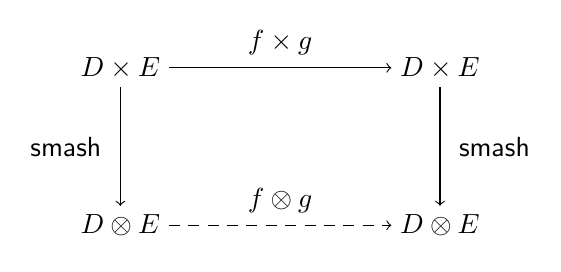
\begin{tikzpicture}[
  x=1cm, y=1cm,
  every node/.style={inner sep=1pt},
  open/.style={circle, draw, fill=white, minimum size=4pt, inner sep=0pt},
  solid/.style={circle, draw, fill=black, minimum size=5pt, inner sep=0pt},
  edge/.style={draw, line width=0.4pt},
  % added for the commutative diagrams: object nodes, and the paper's two
  % arrow kinds -- solid for a named map, dashed for the unique completing map
  obj/.style={inner sep=3pt},
  arrow/.style={draw, line width=0.4pt, ->},
  darrow/.style={draw, line width=0.4pt, ->, dash pattern=on 4pt off 3pt}]

  % vertices
  \node[obj] (tl) at (0.00,2.00) {$D \times E$};
  \node[obj] (tr) at (4.06,2.00) {$D \times E$};
  \node[obj] (bl) at (0.00,0.00) {$D \otimes E$};
  \node[obj] (br) at (4.06,0.00) {$D \otimes E$};

  % arrows
  \draw[arrow]  (tl) -- (tr);
  \draw[arrow]  (tl) -- (bl);
  \draw[arrow]  (tr) -- (br);
  \draw[darrow] (bl) -- (br);

  % labels printed inside the picture
  \node[anchor=south] at (2.03,2.12) {$f \times g$};
  \node[anchor=south] at (2.03,0.12) {$f \otimes g$};
  \node[anchor=east]  at (-0.20,1.00) {\textsf{smash}};
  \node[anchor=west]  at (4.26,1.00) {\textsf{smash}};
\end{tikzpicture}
\end{document}
